%
% Szakdolgozatminta az Eszterházy Károly Katolikus Egyetem
% matematika illetve informatika szakos hallgatóinak.
%

\documentclass[
% opciók nélkül: egyoldalas nyomtatás, elektronikus verzió
% twoside,     % kétoldalas nyomtatás
% tocnopagenum,% oldalszámozás a tartalomjegyzék után kezdődik
]{thesis-ekf}
\usepackage[T1]{fontenc}
\usepackage{hulipsum}
\PassOptionsToPackage{defaults=hu-min}{magyar.ldf}
\usepackage[magyar]{babel}
\usepackage{mathtools,amssymb,amsthm,pdfpages}
\footnotestyle{rule=fourth}

\newtheorem{tetel}{Tétel}[chapter]
\theoremstyle{definition}
\newtheorem{definicio}[tetel]{Definíció}
\theoremstyle{remark}
\newtheorem{megjegyzes}[tetel]{Megjegyzés}

\begin{document}
	\institute{Matematikai és Informatikai Intézet}
	\title{Programozható elektronikák alkalmazásai}
	\author{Bagoly Gábor\\programtervező informatikus}
	\supervisor{Dr. Geda Gábor\\egyetemi docens}
	\city{Eger}
	\date{2023}
	\maketitle
	\tableofcontents
	
	\chapter*{Bevezetés}
	\addcontentsline{toc}{chapter}{Bevezetés}
	
	A mai világunkban az okos otthonok és az okos eszközök rendkívül népszerűek és elterjedtek lettek. Általában, hogy ha megkérdezünk valakit ezzel a témával kapcsolatban, akkor nagy valószínűséggel azt tudják elmondani, hogy rendelkeznek legalább egy okos otthonban alkalmazható eszközzel.
	
	Az okos otthonok és az okos eszközök lehetővé teszik a tulajdonosaik számára, hogy akár távolról is vezéreljék és felügyeljék az otthonukat. Ezek az eszközök lehetővé tehetik a kényelmesebb és hatékonyabb életmód megvalósítását. Az okos otthonok és az okos eszközök segítségével például távolról is bekapcsolhatjuk a világítást, beállíthatjuk a fűtést, és megfigyelhetjük a biztonsági kamerákat.
	
	Manapság már ha valaki az interneten rákeres valamilyen otthoni eszközre, és eléje írja azt hogy 'okos', akkor bizonyára léteznek már erre megoldások. - például okos WC-k, okos kenyérpirítók, még akár okos szőnyegek is, és még sorolhatnám ezt a listát tovább. 
	
	De mi is tesz egy eszközt okossá? Feltételezhetjük azt, hogy ha valami internetre kapcsolódik, esetleg távolról beállíthatjuk, vagy automatizálhatjuk előre meghatározott dolgokra, akkor azt az eszközt ,,okosnak'' tudjuk mondani.
	
	Hogy ha valaki már rendelkezik több ilyen eszközzel, akkor bizonyára találkoztak már azzal a problémával, hogy az egy bizonyos ökoszisztémában használatos eszközök nem feltétlenül tudnak működni egy másikban. Minderre próbáltam egy olyan megoldást kitalálni, ami abból a szempontból közelíti meg, hogy még egy 'nem okos' eszközt (például egy izzót) integrálok bele úgy a rendszerbe, hogy ezt egyszerűen tudjunk kezelni bárhonnan az otthonunkból, ehhez társulva különböző programozható elektronikák. Mindehhez egy olyan webes alkalmazást hoztam létre, amely felelős a háttérben lévő folyamatok lebonyolítására, és az általunk ismert legtöbb eszközön alkalmazható, amin internetezni is tudunk: legyen az számítógép, Androidos, vagy iOS-es telefon, tablet, vagy akár okos óra is.
	
	Azért került erre a témára a választásom, mivel számomra felettébb érdekes az, hogy egy ilyen okos otthonban az eszközök hogyan is kommunikálnak, és szeretnék ebbe egy belátást nyerni, hogy hogyan is épül össze mindez.

	Célom az lenne ezzel, hogy belelássak egy ilyen rendszer működésébe, különböző programozható eszközök alkalmazását jobban megismerjem, és, hogy egy olyan általános kezelőfelületet tudjak létrehozni, amit könnyen tud a felhasználó alkalmazni.
	
	\chapter{Piacon lévő okos otthon rendszerek}
	\section{Nagyobb cégek által létrehozott ökoszisztémák}
		Az okos otthon rendszerek széles választéka áll rendelkezésre a piacon felhasználók számára, amelyek között egyszerű rendszerektől kezdve a biztonsági kamerák, ajtózárak és akár a háztartási készülékek is alkalmazhatóak. Amikor az okos otthon rendszer kiválasztására kerül sor, fontos figyelembe venni az eszközök kiválasztását is.
		
		Van néhány olyan eszköz, - például okos izzók vagy okos dugaljak -, amelyek több okos otthon rendszerrel is szabadon használhatóak, így könnyen integrálhatóak a választott rendszerbe. Ezek az eszközök általában ipari szabványokat használnak, mint például a Wi-Fi, Bluetooth LE vagy a Zigbee, ami lehetővé teszi számukra, hogy kommunikáljanak a különböző okos otthon rendszerekkel.
		
		Azonban vannak olyan eszközök is, amelyek kifejezetten egyetlen rendszerrel működnek együtt. Ezek az eszközök saját protokollokat vagy szoftvereket használhatnak, amelyek nem kompatibilisek más rendszerekkel, ami korlátozhatja az okos otthon rendszerünk rugalmasságát. Vegyük példának azt, hogy ha olyan okos ajtózárat vásárlunk, amely csak egy meghatározott okos otthon rendszerrel működik együtt, akkor az eszközt később nem tudjuk használni egy másik rendszerrel. Vagy hogy ha veszünk egy adott típusú eszközt, akkor azt későbbiekben nem tudjuk kombinálni egy másik rendszer eszközével.
		
		Összességében az okos otthon eszközök kiválasztásakor fontos figyelembe venni a kompatibilitást választott okos otthon rendszerünkkel. Az iparági szabványokat támogató eszközök általában rugalmasabbak és szélesebb körű rendszerekkel használhatóak, míg a saját protokollokat használó eszközök korlátozottabbak lehetnek a kompatibilitás terén.
		
	\subsection*{Amazon rendszere - Amazon Alexa és az Amazon Echo}
	2014-ben robbant be a piacra az Amazon - \emph{az akkor még újdonságnak számító} - okos hangszórójukkal, az Amazon Echo-val. Ekkor még leginkább csak annyira volt képes, hogy a felhasználó zenét tudja irányítani hang utasításokkal. Ez az eszköz úgy működik, hogy ebbe bele van integrálva az Amazon sajátos virtuális asszisztense, amit Alexának hívnak. Ugye mint kezdetleges szoftver, neki sem voltak a képességei túl szerteágazóak. Leginkább arra tudta az ember használni, hogy egyszerű kérdéseket tegyen fel az ember, és zenét tudjon elindítani, leállítani átugrani.
	
	Nem is annyira később, amikor elkezdett egyre jobban fejlődni Alexa, úgy egyre több mindenre kezdhette el használni az ember: termosztátok beállítása, izzók ki- és bekapcsolására is már lehetett használni. Miután az Amazon egyre többet fektetett bele a rendszerükbe felettébb szerteágazó lett annak a használata az otthonokban. Még arra is volt lehetőség már ekkor, hogy akár bevásárló listát készítsen, és azokat meg is tudja rendelni a felhasználó az Amazonról, mindezt Alexa használatával. A cég 2017 május 23-án jelentette be, hogy a \emph{Smart Home Skill API}-jukba\footnote{A blog poszt amiben bejelentették a Smart Home Skill API bővítését\cite{amazon-api}} innentől kezdve megadható, hogy milyen eszközöket is csatlakoztatunk a rendszerükbe, ami kitárta a lehetőségeket az otthoni okos készülékek automatizációjára. Mindezek mellett ezzel egye jobban elkezdett növekedni az okos otthon piac, és az ehhez tartozó virtuális asszisztensek szerepe. Az Amazon által szolgáltatott okos otthon rendszer 2023-ra olyan szintre jutott, hogy az Amerikai Egyesült Államokban az ilyen hang vezérelt hangszórók 68.2\%-a az Amazon Echo.\footnote{Statisztikai adatokat az Earthweb: ,,How Many People Use Alexa in 2023? (U.S. Amazon Statistics)'' cikkjéből \cite{amazon-stats}} 

	
	\subsection*{Google rendszere - Google Home}
	
	\subsection*{Xiaomi rendszere - Mi Home}
	
	\subsection*{Apple rendszere - Apple HomeKit}
	
	\subsection*{Samsung rendszere - Samsung SmartThings}
	
	\section{Nyílt forrású, szabadon személyre szabható rendszerek}
	\subsection*{Mit jelent az, hogy open source?}
	
	\subsection*{Home Assistant}
	
	\subsection*{OpenHAB}
	
	\subsection*{Domoticz}
	
	\subsection*{Calaos}
	%----------
	\chapter{Alkalmazott eszközök}
	\section{Hardver}
	\subsection{Raspberry Pi 4B}
	\subsection{ESP-Wroom-32 - Wi-Fi-s Mikrokontroller}
	\subsection{ESP32-CAM - Wi-Fi-s kamera modul}
	\subsection{DHT22 - hőmérséklet és páratartalom szenzor}
	\subsection{RFID-RC522 - RFID olvasó + RFID technológia összefoglaló}
	\subsection{Szolidtest relé}
	\subsection{Eszközök bekötése - Fritzing}
	
	\section{Szoftver - Programozási nyelvek}
	\subsection{C++ - Arduino IDE}
	\subsection{HTML - PHP Storm}
	\subsection{PHP - PHP Storm}
	\subsection{JavaScript, ChartJS, jQuery - PHP Storm}
	\subsection{Tailwind}
	\subsection{dbDiagram}
	\subsection{font-awesome}
	\subsection{MySQL}
	\subsection{plantUML}
	\section{Laravel}
	\subsection{Laravel működése}
	%----------
	
	\chapter{A web alkalmazás felépítése és működése}
	\section{Raspberry PI4B alkalmazása, mint Wi-Fi, és hub}
	\section{Adatbázis felépítése}
	\section{Kezelő felület bemutatása és működése}
	\subsection{Főoldal}
	\subsection{Beállítások}
	\subsection{RFID beállítások}
	\subsection{RFID használati táblázat}
	\subsection{Hőmérsékleti és páratartalom előzmények - ChartJS}
	\section{Eszközök kommunikációja a webszerverrel}
	
	%----------
	\chapter{Tesztelések}
	\section{Tesztelések módjai és fontossága}
	
	\subsection{Cypress automatizált tesztelések}
	\subsection{Manuális tesztelések}
	\begin{table}[h]
		\centering
		\begin{tabular}{|p{6cm}|p{6cm}|p{4cm}|}
			\hline
			\textbf{Teszt leírása} & \textbf{Elvárt eredmények} & \textbf{Tapasztalatok} \\
			\hline
			Access Control Test: RFID tags assigned to users &
			 The system should recognize the RFID tags assigned to each user and grant or deny access to specific devices or areas of the home accordingly &
			  The test was successful, with the system accurately recognizing and responding to each user's assigned RFID tag \\
			\hline
			Device Control Test: Using RFID tags to control devices &
			 The system should allow users to control smart home devices (such as lights or locks) using RFID tags, without requiring additional input &
			  The test was partially successful, with the system accurately recognizing the RFID tags but experiencing some delays in device response times \\
			\hline
			Durability Test: RFID tags in high traffic areas &
			 The RFID tags should remain functional and readable even in high traffic areas, with no degradation in performance &
			  The test was successful, with the RFID tags remaining fully functional and readable even with heavy usage \\
			\hline
			Security Test: Unauthorized access prevention &
			 The system should be designed to prevent unauthorized access by detecting and alerting the user to the presence of unrecognized RFID tags & 
			 The test was successful, with the system detecting and preventing access by an unrecognized RFID tag, and sending an alert to the user's mobile device \\
			\hline
		\end{tabular}
		\caption{Manuális tesztelések a webalkalmazásra}
		\label{table:manual-testing-results}
	\end{table}
	
	%----------
	\chapter{Rendszer telepítése}

	
	\chapter*{Összegzés}
	\addcontentsline{toc}{chapter}{Összegzés}
	
	\begin{thebibliography}{20}
		\addcontentsline{toc}{chapter}{\bibname}
		
		\bibitem{amazon-api}
		\textsc{Jeff Blankenburg}: \emph{Define Your Appliance Category for a Better Customer Experience}\\
		\textsc{URL:} \url{https://developer.amazon.com/blogs/alexa/post/a89f7243-08a0-4c73-8fc5-eb604a93f437/define-your-appliance-category-for-a-better-customer-experience?asc_refurl=https%3A%2F%2Fwww.businessinsider.com%2F&asc_source=browser&asc_campaign=commerce-pra&tag=thebusiinsi-20}
		
		\bibitem{amazon-stats}
		\textsc{Jason Wise}: \emph{How Many People Use Alexa in 2023? (U.S. Amazon Statistics)} 
		\textsc{URL:} \url{https://earthweb.com/alexa-users/}
		
		\bibitem{openSource}
		\textsc{What is open source}\\
		\textsc{URL:} \url{https://opensource.com/resources/what-open-source}
		
		\bibitem{closed-sh-gateway}
		\textsc{Breaking Down the Compatibility Problem in Smart Homes: A Dynamically Updatable Gateway Platform}\\
		\textsc{URL:} \url{https://www.ncbi.nlm.nih.gov/pmc/articles/PMC7285766/}
		
		\bibitem{top7-opensource-homes}
		\textsc{Top 7 Open Source Home Automation Software}\\
		\textsc{URL:} \url{https://fixthephoto.com/best-open-source-home-automation-software.html}
		
		\bibitem{what-is-smarthome}
		\textsc{What is the Smart Home?}\\
		\textsc{URL:} \url{https://shaba.eu/2020/11/03/what-is-the-smart-home/}
		
		\bibitem{evolution-of-smarthome}
		\textsc{Nathan Hart}: \emph{The Evolution of the Smart Home: How it Started [Part 1]}\\
		\textsc{URL}: \url{https://ubuntu.com/blog/the-evolution-of-the-smart-home-how-it-started-part-1}
		
		\bibitem{smart-home}
		\textsc{Smart Home: Architecture, Technologies and Systems}: \emph{Min Li, Wenbin Gu, Wei Chen, Yeshen He, Yannian Wu, Yiying Zhang}\\
		\textsc{URL:} \url{https://www.sciencedirect.com/science/article/pii/S1877050918305994?via%3Dihub}
		
		\bibitem{smart-home-definition}
		\textsc{Forrest Stroud}: \emph{Smart Home}\\
		\textsc{URL:} \url{https://www.webopedia.com/definitions/smart-home/}
		
		\bibitem{raspberrypi-4b}
		\textsc{Offical Raspberry Pi 4B dokumentation}\\
		\textsc{URL:} \url{https://www.raspberrypi.com/documentation/computers/raspberry-pi.html#raspberry-pi-4}
		
		\bibitem{ESP32-devices}
		\textsc{Offical ESP32 devices documentation}\\
		\textsc{URL:} \url{http://esp32.net/#Info}
		
		\bibitem{esp32-wroom}
		\textsc{NodeMCU ESP-WROOM-32 internal details and pinouts}\\
		\textsc{URL:} \url{https://www.instructables.com/ESP32-Internal-Details-and-Pinout/}
		
		\bibitem{RFID-card-reader}
		\textsc{Connect RFID to PHP \& MySQL Database with NodeMcu ESP8266}\\
		\textsc{URL:} \url{https://iotprojectsideas.com/connect-rfid-to-php-mysql-database-with-nodemcu-esp8266/}
		
		\bibitem{node32-httpget}
		\textsc{ESP8266 NodeMCU HTTP GET and HTTP POST with Arduino IDE (JSON, URL Encoded, Text)}\\
		\textsc{URL:} \url{https://randomnerdtutorials.com/esp8266-nodemcu-http-get-post-arduino/#http-get-1}
		
		\bibitem{arduino-to-laravel}
		\textsc{Arduino to Laravel Communication}\\
		\textsc{URL:} \url{https://www.instructables.com/Arduino-to-Laravel-Communication/}
		
		\bibitem{raspberry-as-wifi}
		\textsc{Raspberry configuration for Wi-Fi}\\
		\textsc{URL:} \url{https://www.raspberrypi.com/documentation//computers/configuration.html#setting-up-a-routed-wireless-access-point}
		
		\bibitem{laravel-docs}
		\textsc{Offical Laravel Documentation}\\
		\textsc{URL:} \url{https://laravel.com/docs/10.x}
		
		\bibitem{tailwind-docs}
		\textsc{Offical Tailwind Documentation}\\
		\textsc{URL:} \url{https://tailwindcss.com/docs}
		
		\bibitem{chartjs-docs}
		\textsc{Offical Chart.js Documentation}\\
		\textsc{URL:} \url{https://www.chartjs.org/docs/latest/}
			
		\bibitem{cypress-docs}
		\textsc{Offical Cypress Documentation}\\
		\textsc{URL:} \url{https://docs.cypress.io/guides/overview/why-cypress}
		
		\bibitem{fontawesome}
		\textsc{Fontawesome - Free Icons}\\
		\textsc{URL:} \url{https://fontawesome.com/search?o=r&m=free}
				
	\end{thebibliography}
	
	% Aláírt, szkennelt nyilatkozat beillesztése a szakdolgozat végére
	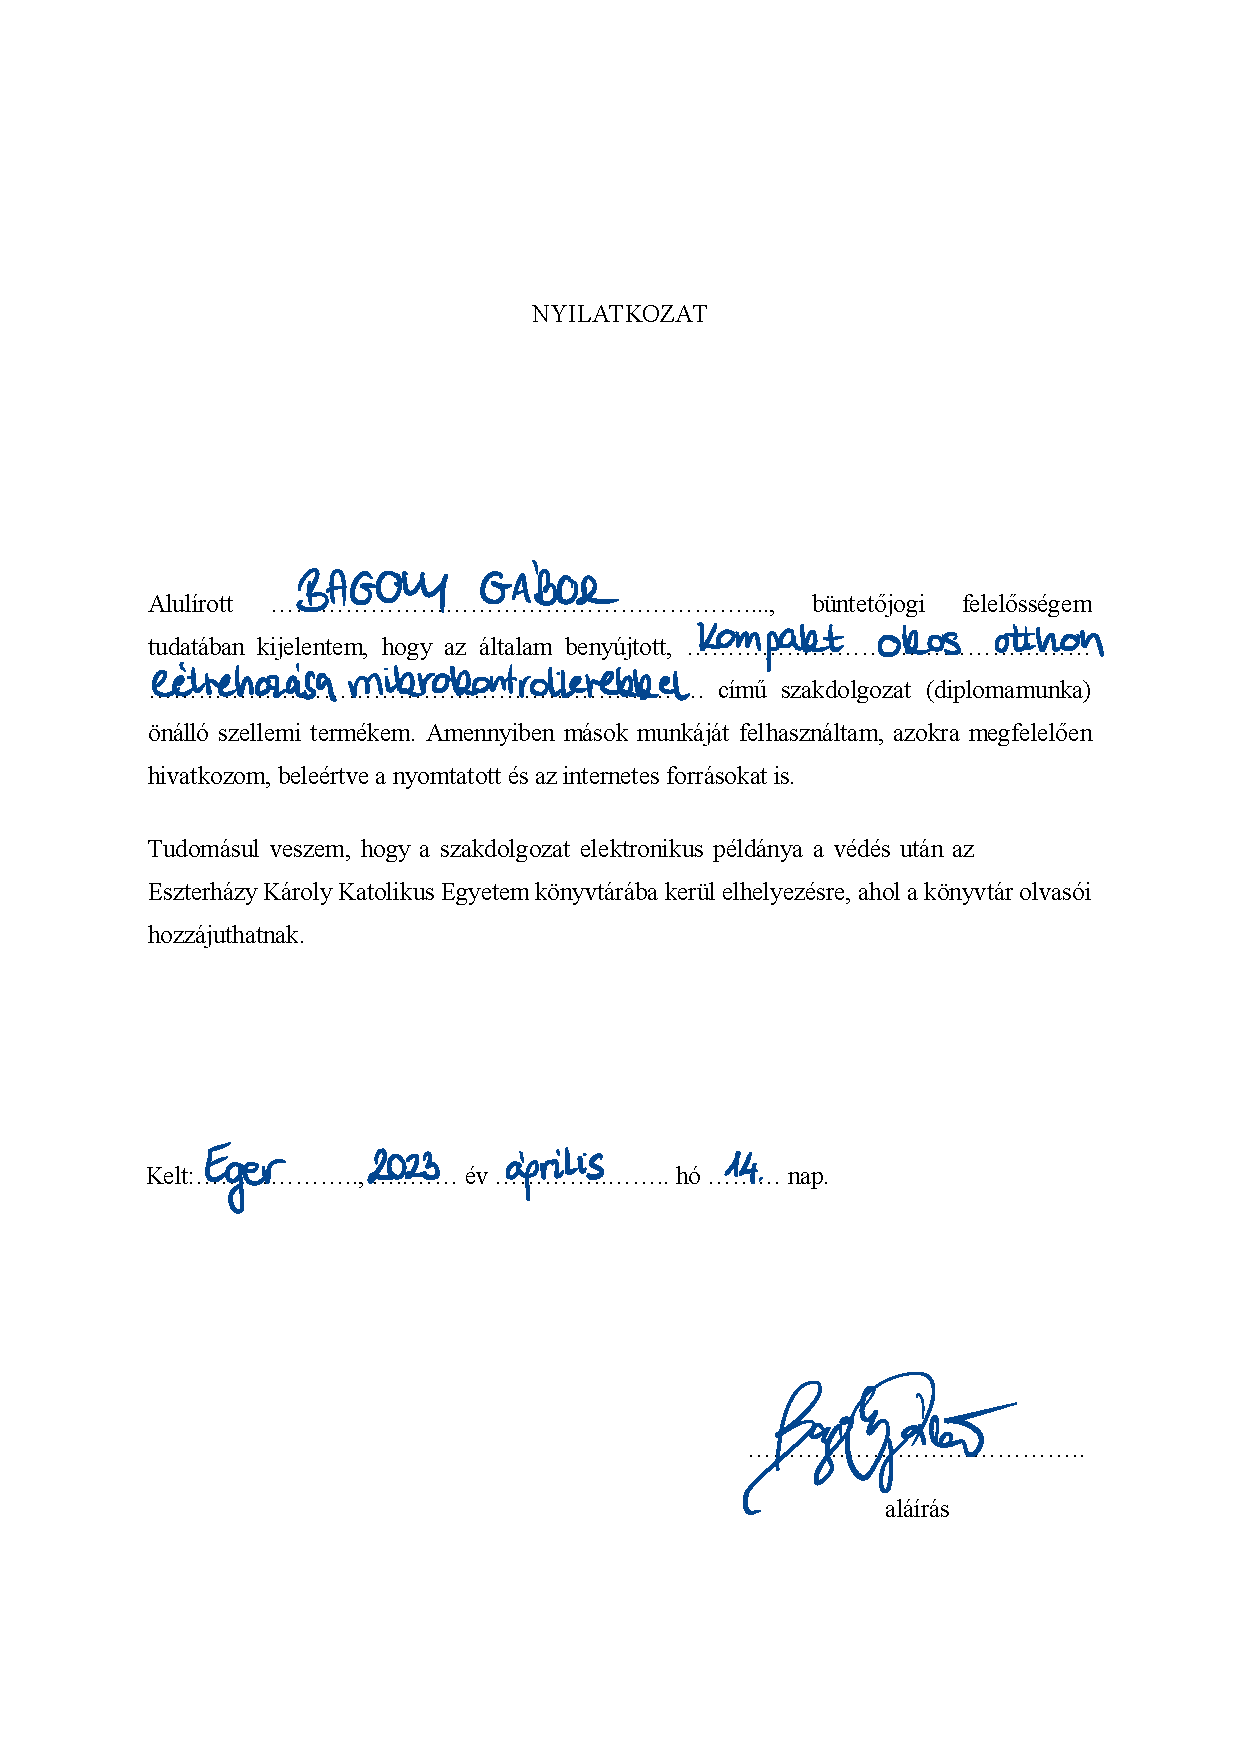
\includepdf{nyilatkozat.pdf}
\end{document}